\section{Referencial Teórico}
\subsection{Compiladores}
Segundo \citeonline{new-dragon-pt}, \compilador é um programa que traduz um
programa-fonte para um programa-objeto. Se o programa-objeto for executável,
então ele estará num formato que um computador possa executá-lo. Dessa forma, um compilador recebe
como entrada um arquivo contendo um programa escrito em uma linguagem previamente
determinada (programa-fonte) e produz como saída um programa objeto semanticamente equivalente
ao programa recebido como entrada. Dessa forma, podemos dizer que um \compilador é,
também, um tradutor. Adicionalmente o \compilador tem como tarefa reportar os
erros encontrados durante o processo de tradução.

O \compilador pode ser dividido em alguns módulos para efetuar o processo de
tradução. A lista abaixo foi proposta por \citeonline{louden97-pt}:

\begin{itemize}
	\item Analisador Léxico;
	\item Analisador Sintático;
	\item Analisador Semântico;
	\item Gerador de Código.
\end{itemize}

O \emph{Analisador Léxico} é o responsável por agrupar os caracteres, contidos
no arquivo do programa-fonte, em unidades significativas, chamadas
\emph{tokens}, e encaminhá-las para o \emph{Analisador Sintático}.

Por sua vez, o \emph{Analisador Sintático} verifica se o fluxo de tokens
recebidos pelo Analisador Léxico é válido para a gramática (ou linguagem) que
foi definida. Usualmente o Analisador Sintático produz uma estrutura
(tipicamente uma do tipo árvore) que representa o programa fonte
\cite{new-dragon-pt}.

O \emph{Analisador Semântico} recebe a estrutura produzida pelo Analisador
Sintático e, principalmente, verifica se as operações são coerentes para os
tipos de dados utilizados e faz a inferência dos tipos de dados. Ao final do
processo temos uma \emph{Árvore Anotada}. As notas (informações de inferência,
por exemplo) podem ser incluídas diretamente na estrutura recebida do
Analisador Sintático, ou numa estrutura auxiliar como uma \emph{Tabela de
Símbolos}.

Estando a Árvore Anotada disponível para o \emph{Gerador de Código}, este
executa a tradução das estruturas recebidas para o programa-objeto. Nessa fase
da compilação podem ser incluídas otimizações para que o programa traduzido
execute de forma mais eficiente.

Podem haver outras fases intermediárias durante o processo, como, por exemplo,
as fases de Otimização de Código, dependentes ou não da máquina-alvo.

Nas próximas Seções, discutiremos mais profundamente cada uma dessas etapas
do processo de compilação.

\subsection{Análise Léxica}

O processo de Analise Léxica consiste em agrupar os caracteres do arquivo de
entrada em unidades numa estrutura chamada \token. Um token também é chamado
de \emph{lexema}.

Segundo \citeonline{dict-aurelio}, ``lexema é o elemento que encerra o
significado da palavra''. Ou seja, é o menor conjunto de caracteres
representativos para uma gramática de uma linguagem. Dessa forma, o Analisador
Léxico remove a responsabilidade de representar os tokens do Analisador
Sintático, simplificando sua implementação.

Segundo \citeonline{new-dragon-pt}, os tokens são definidos como segue:

\begin{citacao}{4cm}{0cm}\footnotesize \emph
	Um token consiste em dois componentes, um nome de token e um valor de
	atributo. Os nomes de token são símbolos abstratos usados pelo analisador para
	fazer o reconhecimento sintático. Frequentemente, chamamos esses nomes de
	token de \emph{terminais}, uma vez que eles aparecem como \emph{símbolos
	terminais} na gramática para uma linguagem de programação. O valor do
	atributo, se houver, é um apontador para a tabela de símbolos que contém
	informações adicionais sobre o token. (\ldots).
\end{citacao}

Ainda segundo \citeonline{new-dragon-pt}, o Analisador Léxico possui algumas
atribuições adicionais, como por exemplo, remover espaços em branco e
comentários, efetuar contagem de linhas correlacionando um erro com o número
da linha em que este foi encontrado.

Tipicamente, o Analisador Léxico não gera o todo o fluxo de tokens de uma vez.
Ao invéz disso, a demanda de análise dos tokens fica sob a responsabilidade do
Analisador Sintático, que recebe os tokens ativando uma função disponibilizada
pelo Analisador Léxico \cite{louden97-pt}.

O reconhecimento dos tokens é feito utilizando duas técnicas principais:
\emph{Expressões Regulares e Autômatos Finitos}. Trataremos das Expressões
Regulares na Seção \ref{sec:regex}. Para uma introdução a Teoria dos Autômatos
consulte \citeonline{louden97-pt} e  \citeonline{new-dragon}, para um estudo
mais detalhado, consulte \citeonline{hopcroft01}.

\subsubsection{Expressões Regulares}
\label{sec:regex}

Segundo \citeonline{regex-jargas}:
\begin{citacao}{4cm}{0cm} \footnotesize \emph
	Resumidamente, uma expressão regular é um método formal de se especificar um padrão de texto.

	Mais detalhadamente, é uma composição de símbolos, caracteres com funções
	especiais, que, agrupados entre si e com caracteres literais, formam uma
	sequência, uma expressão. Essa expressão é interpretada como uma regra, que
	indicará sucesso se uma entrada de dados qualquer casar com essa regra, ou
	seja, obedecer exatamente a todas as suas condições
\end{citacao}

As expressões regulares são uma importante notação para especificar os padrões
dos lexemas. Mesmo não podendo especificar todos os padrões possíveis elas são
muito eficientes para o propósito de especificar os tokens que necessitamos.

\textbf{Definições} (segundo \citeonline{new-dragon-pt}):
\begin{description}
	\item[Alfabeto] é qualquer conjunto finito de símbolos. Temos como exemplos
		de símbolos as letras, dígitos etc. O conjunto $\{0, 1\}$ representa o
		\emph{alfabeto binário}.
	\item[Cadeia] em um alfabeto é uma sequência finita de símbolos retirados de
		alfabeto. Normalmente, o tamanho da cadeia $s$ é dado por $|s|$. Por
		exemplo ``compilador'' é uma cadeia de tamanho 10. A cadeia vazia,
		indicada por $\epsilon$, tem tamanho zero.
	\item[Linguagem] é qualquer conjunto contável de cadeias de algum alfabeto.
\end{description}

\textbf{Expressão Regular Básica} são, simplesmente, os caracteres separados do
alfabeto que casam com eles mesmos. Por exemplo, dado que definimos o conjunto
dos caracteres ASCII como nosso alfabeto, a expressão regular $/a/$ casa com o
caractere \textbf{a}.

Há três operações básicas utilizando Expressões Regulares conforme descritas
abaixo \cite{louden97-pt}:

\begin{description}
	\item[Escolha Entre Alternativas] Dado que $r$ e $s$ são expressões
		regulares, então $r | s$ é uma expressão regular que case com a expressão
		$r$ ou com a expressão $s$. Exemplo: dado que $r$ seja a expressão regular
		$/a/$ e $s$ a expressão regular $/b/$, $r | s$ casa com o caractere
		\textbf{a} ou o caractere \textbf{b}.
	\item[Concatenação] A concatenação de duas expressões regulares $r$ e $s$ é
		da pela expressão $rs$ e casa com qualquer cadeia que case com a expressão
		regular $r$ seguida pela expressão regular $s$. Exemplo: dado que $r$ seja
		a expressão regular $/ca/$ e $s$ a expressão regular $/sa/$, $rs$ casa
		com a cadeia ``casa''.
	\item[Repetição] Também conhecida como fecho de Kleene, é denotada por $r*$,
		em que $r$ é uma expressão regular. A expressão regular $r*$ representa o
		conjunto de cadeias obtidas pela concatenação de zero ou mais expressões
		regulares $r$. Exemplo: dada a expressão regular $/a*/$, esta expressão
		casa com as cadeias \textbf{$\epsilon$}, \textbf{a}, \textbf{aa},
		\textbf{aaa}, \textbf{aaaa}, \dots.
\end{description}

Para simplificar a notação das expressões regulares é comum associar nomes às
expressões regulares longas. Uma Expressão Regular nomeada é chamadas de
\textbf{definição regular}.

Além das operações descritas, a norma \citeonline{POSIX.1} define operações
adicionais chamadas Expressões Regulares Extendidas:

\begin{description}
	\item[Uma ou Mais Repetições] A repetição de de uma ou mais vezes da
		expressão regular $r$ é dada por $r+$, eliminando o casamento da expressão
		vazia (\(\epsilon\)). O mesmo resultado poderia ser obtido com a expressão
		$rr*$, mas esta é uma situação tão frequente que foi simplificada e
		padronizada \cite{louden97-pt}.
	\item[Qualquer Caractere] Um ``.'' (ponto) é utilisado para efetuar o
		casamento com qualquer caractere, exceto um caractere nulo.
\end{description}

Há outras operações que envolvem expressões regulares. Para mais informações
consulte \citeonline{regex-jargas}, \citeonline{POSIX.1} e
\citeonline{louden97-pt}.


\subsection{Análise Sintática}

A Análise Sintática define a forma com que um programa é estruturado. Essa
estrutura é dada por um conjunto de \emph{regras gramaticais} descritas em uma
\emph{Gramática Livre de Contexto} (verificar Seção \ref{sec:context_free_grammar}).

Segundo \citeonline{new-dragon-pt}:
\begin{citacao}{4cm}{0cm}\footnotesize \emph
	Existem três estratégias gerais de análise sintática para o processamento
	de gramáticas: universal, descendente e ascendente. Os métodos de análise
	baseados na estratégia universal (\dots) podem analisar qualquer
	gramática, (\dots) no entanto são muito ineficientes para serem utilizados
	em compiladores de produção.

	Os métodos geralmente usados em compiladores são baseados nas estratégias
	descendentes ou ascendentes. Conforme sugerido por seus nomes, os métodos
	de análise descendentes constroem as árvores de derivação de cima (raiz)
	para baixo (folhas), enquanto os métodos ascendentes fazem a análise no
	sentido inverso, começam nas folhas e avançam até a raiz construindo a
	árvore. Em ambas as estratégias, a entrada do analisador sintático é
	consumida da esquerda para a direita, um símbolo de cada vez.
\end{citacao}

Para maiores referências sobre analisadores descendentes (descendente
recursivos e LL(k)), consulte \citeonline{louden97-pt}, \citeonline{parr07},
\citeonline{jacobs85}.

\subsubsection{Gramáticas Livres de Contexto}
\label{sec:context_free_grammar}

\emph{Gramática} é essencialmente um conjunto de Regras de Produção (ou
Re-escrita). Essas regras são, usualmente, descritas utilizando uma notação
chamada \textbf{Forma de Backus-Naur}, ou \textbf{BNF} \cite{louden97-pt}.

Um exemplo abstrato de regra de produção é demonstrado abaixo:

\[
A \rightarrow \alpha
\]

Esta expressão indica que o não-terminal \(A\) será substituído pela sequência
de terminais e/ou não-terminais representada por \(\alpha\). Um \emph{terminal},
normalmente, é um \emph{token} oriundo do analisador léxico.

Um exemplo mais concreto é demonstrado abaixo:

\[
expr \rightarrow expr + expr | \textbf{numero}
\]

Esta regra indica que uma expressão é composta de uma expressão seguida de um
sinal de + seguida de outra expressão, ou de um número. O nome da regra é dado
pela parte que está a esquerda da seta, seu corpo é dado pelo que está a
direita. O sinal \(|\) indica uma escolha de alternativas no corpo da
produção. Percebemos, também, que uma regra gramatical pode ter uma
definição recursiva.

Segundo \citeonline{louden97-pt}, podemos definir uma \textbf{gramática livre de
contexto} mais formalmente conforme segue:
\begin{enumerate}
	\item Um conjunto \(T\) de \textbf{terminais}.
	\item Um conjunto \(N\) de \textbf{não-terminais} (disjunto de \(T\)).
	\item Um conjunto \(P\) de \textbf{produções} na forma \(A \rightarrow \alpha\)
				em que \(A\) é um elemento de \(N\) e \(\alpha\) é um elemento de
				\((T \cup N)^*\) (uma sequência de terminais e não-terminais que
				pode ser vazia).
	\item Um \textbf{símbolo inicial} \(S\) do conjunto \(N\).
\end{enumerate}

Dessa forma, o processo de reconhecimento da linguagem inicia-se derivando o
símbolo inicial da gramática, substituindo repetidamente um não-terminal pelo
corpo desse não terminal \cite{new-dragon-pt}.

Assim, uma \textbf{gramática livre de contexto} é uma \emph{gramática}
conforme definido a cima, e é livre de contexto pois a parte a esquerda de uma
regra de produção pode ser substituída pelo seu corpo em qualquer ponto,
independentemente de onde ocorra a parte esquerda da regra \cite{louden97-pt}.

Em contrapartida, uma produção em uma gramática sensível ao contexto é demonstrada
abaixo:
\[
	\gamma{}A{}\beta \rightarrow \gamma\alpha\beta
\]

Nesta regra, \(A\) pode ser substituído por \(\alpha\), somente se
\(A\) estiver entre os terminais \(\gamma\) e \(\beta\).

\subsubsection{Análise Sintática Ascendente}
\label{sec:asc_syntax_analisys}
O processo de análise sintática ascendente foi proposto por Donald E. Knuth
em 1965. Em seu artigo, ele define a análise sintática $\textbf{LR(k)}$. O
``L'' indica que a entrada é processada da esquerda para a direita e o ``R''
indica que uma derivação a direita é produzida, e a variável $k$ indica
o número de símbolos de verificação a frente utilizados pelo analisador.
\cite{louden97-pt}.

Ainda segundo \citeonline{louden97-pt}, essa forma de análise foi
considerada impraticável até que as técnicas \emph{SLR} e \emph{LALR}
foram desenvolvidas por DeRemer em 1969. Ainda assim, não é prática usual
construir um analisador sintático ascendente manualmente, mas utilizar um
gerador que abstraia os detalhes de implementação (Verificar Seção
\ref{sec:yacc}). Mais detalhes sobre essas técnicas podem ser obtidos em
\citeonline{knuth65}, \citeonline{Deremer69}, \citeonline{new-dragon-pt}.

Os analisadores ascendentes utilizam uma pilha explícita (diferentemente dos
analisadores recursivos, que utilizam a pilha implicitamente) durante o processo de
análise sintática e, no geral, possuem duas ações possíveis, além da aceitação:

\begin{enumerate}
	\item \textbf{Carregar} um terminal da entrada para o topo da pilha.
	\item \textbf{Reduzir} uma cadeia de terminais $\alpha$ para um não-terminal
	      $A$, dada a escolha da regra $A \rightarrow \alpha$.
\end{enumerate}

Por causa dessa duas ações possíveis, esse tipo de analisador também é
conhecido como \textbf{carrega-reduz} (ou \emph{shift-reduce}).

\begin{lstlisting}[label=lst:grammar_example, caption=Gramática Exemplo]
expressao = termo
          ;

termo = termo + termo
      | termo - termo
      | fator
      ;

fator = fator * fator
      | (termo)
      | numero
      ;
\end{lstlisting}

\begin{lstlisting}[label=lst:source_example, caption=Programa Exemplo]
10 * 20 + 30
\end{lstlisting}

Dados a gramática exemplo da Listagem \ref{lst:grammar_example} e o programa
da Listagem \ref{lst:source_example}, e considerando os símbolos $T$, $F$ como
os não-terminais \emph{termo}, \emph{fator} e $N$ como o terminal \emph{numero},
respectivamente, que \emph{numero} representa um número inteiro, teremos os
seguintes passos executados pelo analisador sintático:

\begin{enumerate}
  \item Carregar $N$ na pilha.
  \item Reduzir o topo da pilha para $F$ e empilhar.
  \item Carregar o token ``*'' na pilha.
  \item Carregar o token $N$ na pilha.
  \item Reduzir o topo da pilha para $F$ e empilhar.
  \item Reduzir $F*F$ para $F$.
	\item Reduzir $F$ para $T$
  \item Carregar o token ``+'' na pilha.
  \item Carregar o token $N$ na pilha.
  \item Reduzir $N$ para $F$ e empilhar.
  \item Reduzir $F$ para $T$ e empilhar.
  \item Reduzir $T+T$ para $T$.
	\item Reduzir $T$ para \emph{expressao}.
\end{enumerate}

Nesse momento, o analisador sintático retorna informando que o programa está
correto, que a sequência de tokens foi aceita como válida para a gramática
definida. Mais detalhes de como são feitas as escolhas entre \emph{carregar} um token
e escolher a regra para efetuar uma \emph{redução} podem ser encontradas em
\citeonline{new-dragon-pt}

\subsubsection{Geradores de Analisadores Sintáticos Ascendentes}
\label{sec:yacc}

Conforme citado na Seção \ref{sec:asc_syntax_analisys}, não é usual a
implementação manual de um Analisador Sintático Ascendente. Dessa forma, temos
alguns geradores que simplificam esse processo para o implementador de um
compilador.

Um gerador amplamente utilizado é o \emph{YACC} (do inglês \emph{yet another
compiler compiler {--} ``mais um compilador de compiladores''}
\cite{louden97-pt}.

Segundo \citeonline{yacc}:

\begin{citacao}{4cm}{0cm} \footnotesize \emph
Yacc provides a general tool for imposing structure on the input to a computer
program. The Yacc user prepares a specification of the input process; this
includes rules describing the input structure, code to be invoked when these
rules are recognized, and a low-level routine to do the basic input. Yacc then
generates a function to control the input process. This function, called a
parser, calls the user-supplied low-level input routine (the lexical analyzer)
to pick up the basic items (called tokens) from the input stream. These tokens
are organized according to the input structure rules, called grammar rules;
when one of these rules has been recognized, then user code supplied for this
rule, an action, is invoked; actions have the ability to return values and
make use of the values of other actions.
\end{citacao}

Um arquivo de especificação \emph{YACC} possui o formato básico conforme
o demonstrado na Listagem \ref{lst:yacc_file_format}. Na seção de
\emph{definições}, primeira parte da especificação, é incluído entre os
caracteres \emph{\%\{} e \emph{\%\}} os trechos de código que deverão ser
incluídos diretamente no analisador sintático gerado. Normalmente, são
incluídos nesse ponto da especificação os \emph{headers} necessários, bem
como as declarações de funções auxiliares necessárias.

Ainda na seção de \emph{definições}, são incluídas as definições da união que
armazenará os nós da árvore sintática produzida (verificar Apêndice
\ref{apx:listings} Listagem \ref{parser.y}), dos tokens que estão presentes na
gramática a ser reconhecida, o tipo de retorno dos \emph{não-terminais} e a
precedência dos operadores binários.

\begin{lstlisting}[label=lst:yacc_file_format, caption=Formato Especificação YACC]
{definicoes}
%%
{regras}
%%
{rotinas auxiliares}
\end{lstlisting}

Na seção de \emph{regras}, são definidas as regras sintáticas da gramática.
Para isso é utilizada uma notação BNF. Após a definição de cada regra, é
incluído entre os caracteres \emph{\{} e \emph{\}} um trecho de código em
linguagem C, que representa a \emph{ação semântica} que deverá ser executada
quando aquela regra for encontrada.

Por fim, na seção de \emph{rotinas auxiliares} são incluídas quaisquer funções
que forem necessárias para a execução do analisador sintático. Comumente é
incluída nessa seção a função que informa os erros encontrados pelo analisador
sintático.

\begin{lstlisting}[label=lst:yacc_example, caption=Exemplo de especificação
YACC]
%{
#include <stdlib.h>
#include <stdio.h>

int yylex(void);
int yyerror(const char *, ...);

int resultado;
%}

%union{
	int valor;
}

%token MAIS MENOS VEZES PARD PARE
%token <valor> numero

%%

expressao = termo { resultado = $1; }
          ;

termo = termo MAIS termo  { $$ = $1 + $3 }
      | termo MENOS termo { $$ = $1 - $3 }
      | fator             { $$ = $1 }
      ;

fator = fator VEZES fator { $$ = $1 * $3 }
      | PARE termo PARD   { $$ = $2 }
      | numero            { $$ = yylval.valor }
			;

%%

void yyerror(const char * s, ...) {
  printf("erro de sintaxe: %s\n", s);
  return;
}
\end{lstlisting}

Na Listagem \ref{lst:yacc_example} temos um exemplo concreto de uma
especificação para \emph{YACC}. Foi considerado, para essa especificação, que
o analisador sintático interagiria com o analisador léxico através da chamada
de função \emph{yylex()}. Essa função retorna um inteiro que representa o tipo
de token reconhecido pelo analisador léxico. Em nosso exemplo temos as
representações \textbf{MAIS}, \textbf{MENOS}, \textbf{VEZES}, \textbf{PARE},
\textbf{PARD}, que significam, respectivamente os caracteres \textbf{+},
\textbf{-}, \textbf{*}, \textbf{(}, \textbf{)}.

O token \emph{numero} também é retornado pelo analisador léxico, mas além do
valor de retorno, é disponibilizado na estrutura \emph{yylval} o valor léxico
correspondente ao token. É possível perceber na listagem \ref{lst:yacc_example}
algumas pseudo-variáveis (aquelas iniciadas pelo caractere \emph{\$} nas ações
semânticas). A variável \emph{\$\$} indica o valor retornado pela ação
semântica. As variáveis representadas por \emph{\$n} em que $n \in \{1, 2, 3,
\dotsc\}$ representam os valores retornados por cada não-terminal reconhecido.

Por fim, na seção de \emph{rotinas auxiliares}, é definida a função
\emph{yyerror()} que é ativada quando o analisador sintático encontra algum
erro.

\subsection{Tabela de Símbolos}



\subsection{Geração de Código}
\emph{Geração de Código} é o processo de utilizar todas as informações
geradas durante as fases de \emph{análise} (Léxica, Sintática etc) para
gerar o programa-objeto. Conforme a arquitetura do compilador, é possível
incluir outras etapas intermediárias, conhecidas como \emph{Representações
Intermediárias} (RI), que visam possibilitar otimizações no programa-objeto
gerado \cite{louden97-pt}.

Uma forma possível de RI é conhecida com \emph{código-de-três-endereços}. Este
formato é conhecido desta forma pois possui a seguinte forma de instruções $x
= y \textbf{op} z$, ou seja, do lado direito da atribuição possui apenas um
operador binário, seus operandos e do lado esquerdo a variável que armazena o
resultado da operação. Variações são permitidas para representar, por exemplo,
o sinal de menos unário $x = -y$.

\begin{lstlisting}[label=lst:three_addresses,caption=Código de 3 Endereços]
t1 = c * d
t2 = a + b
t3 = t1 + t2
x = t3
\end{lstlisting}

A Listagem \ref{lst:three_addresses} demonstra um exemplo do
código-de-três-endereços para a expressão $x=a+b+c*d$. As variáveis
$\text{t}i$ para $i \in \{1,2,3\}$ representam variáveis temporárias criadas pelo próprio
compilador.

Para este projeto, não são geradas RIs, apenas os programas-objeto em
\emph{Linguagem C}, que posteriormente podem ser compiladas por um compilador
C, como o \emph{gcc}, gerando um programa executável, e em \emph{Linguagem
DOT} possibilitando a geração de uma representação gráfica do programa.
Mais referências sobre RIs e códigos-de-três-endereços são encontradas em
\citeonline{new-dragon-pt} e \citeonline{louden97-pt}.

Conforme exposto, este projeto de compilador atua como um tradutor entre
linguagens. Uma abordagem semelhante foi utilizada na implementação inicial da
\emph{Linguagem C++}. Este compilador traduzia programas C++ para programas C
para que pudessem, posteriormente, ser compilados por um compilador C
disponível. Assim, podemos considerar o processo de compilação como um
processo de tradução de uma linguagem de nível mais alto para uma outra
linguagem de nível mais baixo, repetindo o  processo até que seja produzido um
programa executável na máquina-alvo \cite{new-dragon-pt}.

A Geração de Código também consiste num processo de linearização das
estruturas de árvores disponibilizadas pelas fases anteriores, transformando,
por exemplo, uma árvore sintática em um programa C, em que as instruções são
escritas linearmente em um arquivo.

A Listagem \ref{lst:code_gen} demonstra uma possível implementação, em
pseudocódigo, de função geradora de código, tendo como base uma árvore
sintática em que cada nó possui até dois filhos. Notamos que a função pode
vistar a árvore em pré-ordem, em ordem e pós-ordem.

\begin{lstlisting}[label=lst:code_gen,caption=Exemplo Gerador de Código]
funcao geraCodigo (no_arvore T)
inicio
	gerar_codigo_preparatorio(T)
	gerar_codigo(T)
	gerar_codigo_preparatorio_filho_esquerda(T->filho_esquerda)
	gerar_codigo_filho_esquerda(T->filho_esquerda)
	gerar_codigo_preparatorio_filho_direita(T->filho_direita)
	gerar_codigo_filho_direita(T->filho_direita)
	gerar_codigo_final(T)
fim
\end{lstlisting}

Com pequenas alterações no código da Listagem \ref{lst:code_gen}, podemos
incluir mais filhos aos nós filhos à árvore $T$, bem como, representar a
construção de quase todas as construções necessárias para produzir o
programa-objeto.


\subsubsection{Linguagem DOT}
\label{sec:impl_gen_dot}

Segundo \citeonline{EGKNW03}:

\begin{citacao}{4cm}{0cm}
Graphviz is a collection of software for viewing and manipulating abstract
graphs. It provides graph visualization for tools and web sites in domains
such as software engineering, networking, databases, knowledge representation,
and bio-informatics
\end{citacao}

Um dos softwares dessa coleção é o compilador \emph{dot}. Segundo
\citeonline{gansner09}:

\begin{citacao}{4cm}{0cm}
\textbf{dot} draws directed graphs. It reads attributed graph text files and
writes drawings, either as graph files or in a graphics format such as GIF,
PNG, SVG, PDF, or PostScript.
\end{citacao}

\textbf{dot} aceita como entrada um arquivo de texto expresso na Linguagem
DOT (verificar \url{http://graphviz.org/content/dot-language}). Essa
linguagem define três tipos principais de objetos: grafos, nós e arestas.
O grafo principal (mais externo) pode ser direcionado (\emph{digraph} {--}
\emph{directed graph}, ou seja, grafo direcionado), ou não-direcionado. Em um
grafo principal, é possível termos um subgrafo (\emph{subgraph}) que permite
a definições de nós e arestas \cite{gansner09}.

Um nó é criado quando o seu nome aparece pela primeira vez no arquivo. As
arestas são criadas quando dois nós são ligados pelo operador de aresta {->}.

Na Listagem \ref{lst:dot_example} temos o exemplo de um grafo escrito em
DOT que após sua compilação com o comando
$$
\text{dot} \quad \text{-Tpng} \quad \text{exemplo\_dot.gv} \quad \text{>}
\quad \text{exemplo\_dot.png}
$$
gerará a representação gráfica demonstrada na Figura \ref{fig:dot_example}.

\lstinputlisting[label=lst:dot_example, caption=Exemplo de Grafo Expresso em DOT]{src_files/dot_example.gv}

\begin{figure}
	\begin{center}
		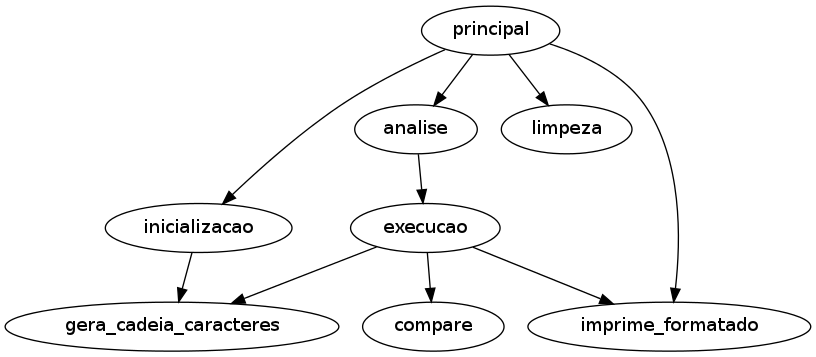
\includegraphics[scale=0.4]{dot_example}
	\end{center}
	\caption{Exemplo Grafo Gerado pelo dot}
	\label{fig:dot_example}
\end{figure}

